\documentclass[a4paper, 16pt]{article}
\usepackage[UTF8]{ctex}
\usepackage{geometry}
\usepackage{graphicx}
\usepackage{setspace}
\usepackage{float}
\usepackage{listings}
\usepackage{xcolor}
\lstset{
    numbers=left, 
    numberstyle= \tiny, 
    keywordstyle= \color{ blue!70},
    commentstyle= \color{red!50!green!50!blue!50}, 
    frame=shadowbox, % 阴影效果
    rulesepcolor= \color{ red!20!green!20!blue!20} ,
    escapeinside=``, % 英文分号中可写入中文
    xleftmargin=2em,xrightmargin=2em, aboveskip=1em,
    framexleftmargin=2em
} 
\geometry{left = 1.0 cm, right = 1.0cm, top = 2.0cm, bottom = 2.0cm	}
\title{编译原理第六章(一)}
\author{李鹏辉}

\begin{document}
\maketitle
1.(6.1.2)为下列表达式构建DAG,且指出它们每个子表达式的值编码。

1) $a+a+(a+a+a+(a+a+a+a))$
\begin{figure}[H]
\centering
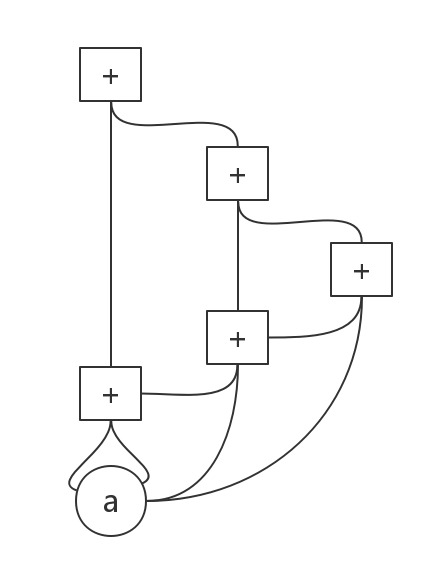
\includegraphics[scale=0.6]{chapter6_hw1_1}
\caption{DAG for the stmt $a+a+(a+a+a+(a+a+a+a))$}
\end{figure}



2.(6.2.1)将算数表达式$a+-(b+c)$翻译成

1)抽象语法树
\begin{figure}[H]
\centering
\includegraphics[scale=0.6]{chapter6_hw1_2}
\caption{DAG for the stmt $a+-(b+c)$}
\end{figure}

2)四元式序列
\begin{table}[H]
\centering
\begin{tabular}{c|c|c|c|c}
\hline
\hline
 &$OP$& $arg1$ & $arg2$ & $result$ \\
\hline
(0) & + & b & c& $t_1$ \\
(1) & uminus & $t_1$ &  & $t_2$\\
(2) & + & $t_1$ & a & $result$ \\
\hline
\end{tabular}
\end{table}

3) 三元式序列
\begin{table}[H]
\centering
\begin{tabular}{c|c|c|c}
\hline
\hline
 &$OP$& $arg1$ & $arg2$ \\
\hline
(0) & + & b & c \\
(1) & uminus & (0)& \\
(2) & + & a & (1) \\
\hline
\end{tabular}
\end{table}
4)间接三元式序列
\begin{table}[H]
\centering
\begin{tabular}{c|c|c|c}
\hline
\hline
 &$OP$& $arg1$ & $arg2$ \\
\hline
(0) & + & b & c \\
(1) & uminus & (0)& \\
(2) & + & a & (1) \\
\hline
\end{tabular}
\end{table}

\begin{table}[H]
\centering
\begin{tabular}{c|c}
\hline
\hline
 &Statement \\
\hline
(0) & (0) \\
(1) & (1) \\
(2) & (2) \\
\hline
\end{tabular}
\end{table}
\end{document}